\documentclass[conference]{IEEEtran}
\IEEEoverridecommandlockouts
% The preceding line is only needed to identify funding in the first footnote. If that is unneeded, please comment it out.
\usepackage{cite}
\usepackage{amsmath,amssymb,amsfonts}
\usepackage{algorithmic}
\usepackage{graphicx}
\usepackage{textcomp}
\usepackage{subfigure}
\usepackage{xcolor}
\def\BibTeX{{\rm B\kern-.05em{\sc i\kern-.025em b}\kern-.08em
    T\kern-.1667em\lower.7ex\hbox{E}\kern-.125emX}}
\begin{document}

\title{Enhancement Techniques for Underwater Images}

\author{\IEEEauthorblockN{Viswanath K}
\IEEEauthorblockA{\textit{Professor, Dept. of ETE} \\
\textit{Siddaganga Institute of Technology}\\
Tumakuru, Karnataka, India \\
vishwanath@sit.ac.in}
\and
\IEEEauthorblockN{Abhilash G}
\IEEEauthorblockA{\textit{Student, Dept. of ETE} \\
\textit{Siddaganga Institute of Technology}\\
Tumakuru, Karnataka, India\\
1si18te001@sit.ac.in}
\and
\IEEEauthorblockN{Pruthveesh R}
\IEEEauthorblockA{\textit{Student, Dept. of ETE} \\
\textit{Siddaganga Institute of Technology}\\
Tumakuru, Karnataka, India\\
1si18te034@sit.ac.in}
\and
\IEEEauthorblockN{Tanmay M}
\IEEEauthorblockA{\textit{Student, Dept. of ETE} \\
\textit{Siddaganga Institute of Technology}\\
Tumakuru, Karnataka, India\\
1si18te050@sit.ac.in}
\and
\IEEEauthorblockN{Tejas V}
\IEEEauthorblockA{\textit{Student, Dept. of ETE} \\
\textit{Siddaganga Institute of Technology}\\
Tumakuru, Karnataka, India\\
1si18te052@sit.ac.in}
}
\maketitle
\begin{abstract}
In this paper, an effective approach for enhancement of underwater images is described. The main source of degradation in underwater images is scattering and absorption in the medium. The foundation of our strategy is on a solitary photograph. This does not require the use of any specialized equipment or specialized knowledge of the topic. The scene's organizational pattern or the situation under the sea expands on what was covered in the earlier study. Merging two images that are immediately created from the same source version of the image that has been adjusted for colour and white balance damaged the original. 
\par
The two pictures are produced by the fusion process, in addition to the weights that are associated with them. The objective of using maps is to improve the way the colours and borders are transferred. In contrast, To complete the image, a detailed weight map was developed. In the signal's low-frequency components, transitions, and variations cause artifacts. In addition to this, we make use of a multi-scale fusion approach. utilizing the images when they were recreated. Our comprehensive approach to qualitative and The results of the quantitative study reveals the following: 
\par
Our newly upgraded visual material now includes several photographs. Dark components have improved visibility, the overall contrast has been enhanced, and the edges now have a greater degree of sharpness. Our investigation has also shown that demonstrates that our method was designed correctly. It is not very unaffected by the settings of the camera and improves several aspects of the precision of the picture processing program. For example, in a picture, two strategies that can be used are segmentation and key point matching. It has the potential to enhance the image's current quality. To validate order to get these improved outcomes, we have employed Peak SNR, Structural Mean Squared Error, as well as the Similarity Index (SSIM) (MSE), in addition to the histogram analysis as quantitative metric analysis.\\
\end{abstract}

\maketitle
\begin{IEEEkeywords}
Image Processing,White Balance,Gamma Correction,Multi-scale Fusion,Normalization.
\end{IEEEkeywords}

\section{Introduction}
Due to poor visibility, little is known about the ocean ecosystems throughout the world. This has to change. Usage of underwater Image enhancing techniques is necessary since 70\% of the Earth's surface is covered by water. Underwater sequences have become more important in the study of marine life, underwater mountains, and flora. Because of this increased interest in what lies under the surface, the necessitates using high-quality pictures, there has been a great demand for Underwater Image Enhancement. The Underwater images were also analyzed for colour impacts. According to Church \cite{WHITE2003693}, light reflection depends heavily on the structure of the water. Another problem is, that light undergoes reflection on the surface of the water and it undergoes Refraction, and dispersion inside the water medium, and when it hits the water molecules light undergoes scattering (Figure 1). So the underwater images look a little bit hazy when compared to images taken in the air. The water's filtering properties, such as dust sprinkling, are heavily influenced by the quality of the water. So while enhancing, we have to make sure these are properly tackled.\\
\begin{figure}
\centering
\includegraphics[width=0.45\textwidth]{3_Effect of Scattering and Absorption.png}
\caption{Effect of Scattering and Absorption}
\end{figure}

\begin{figure}
\centering
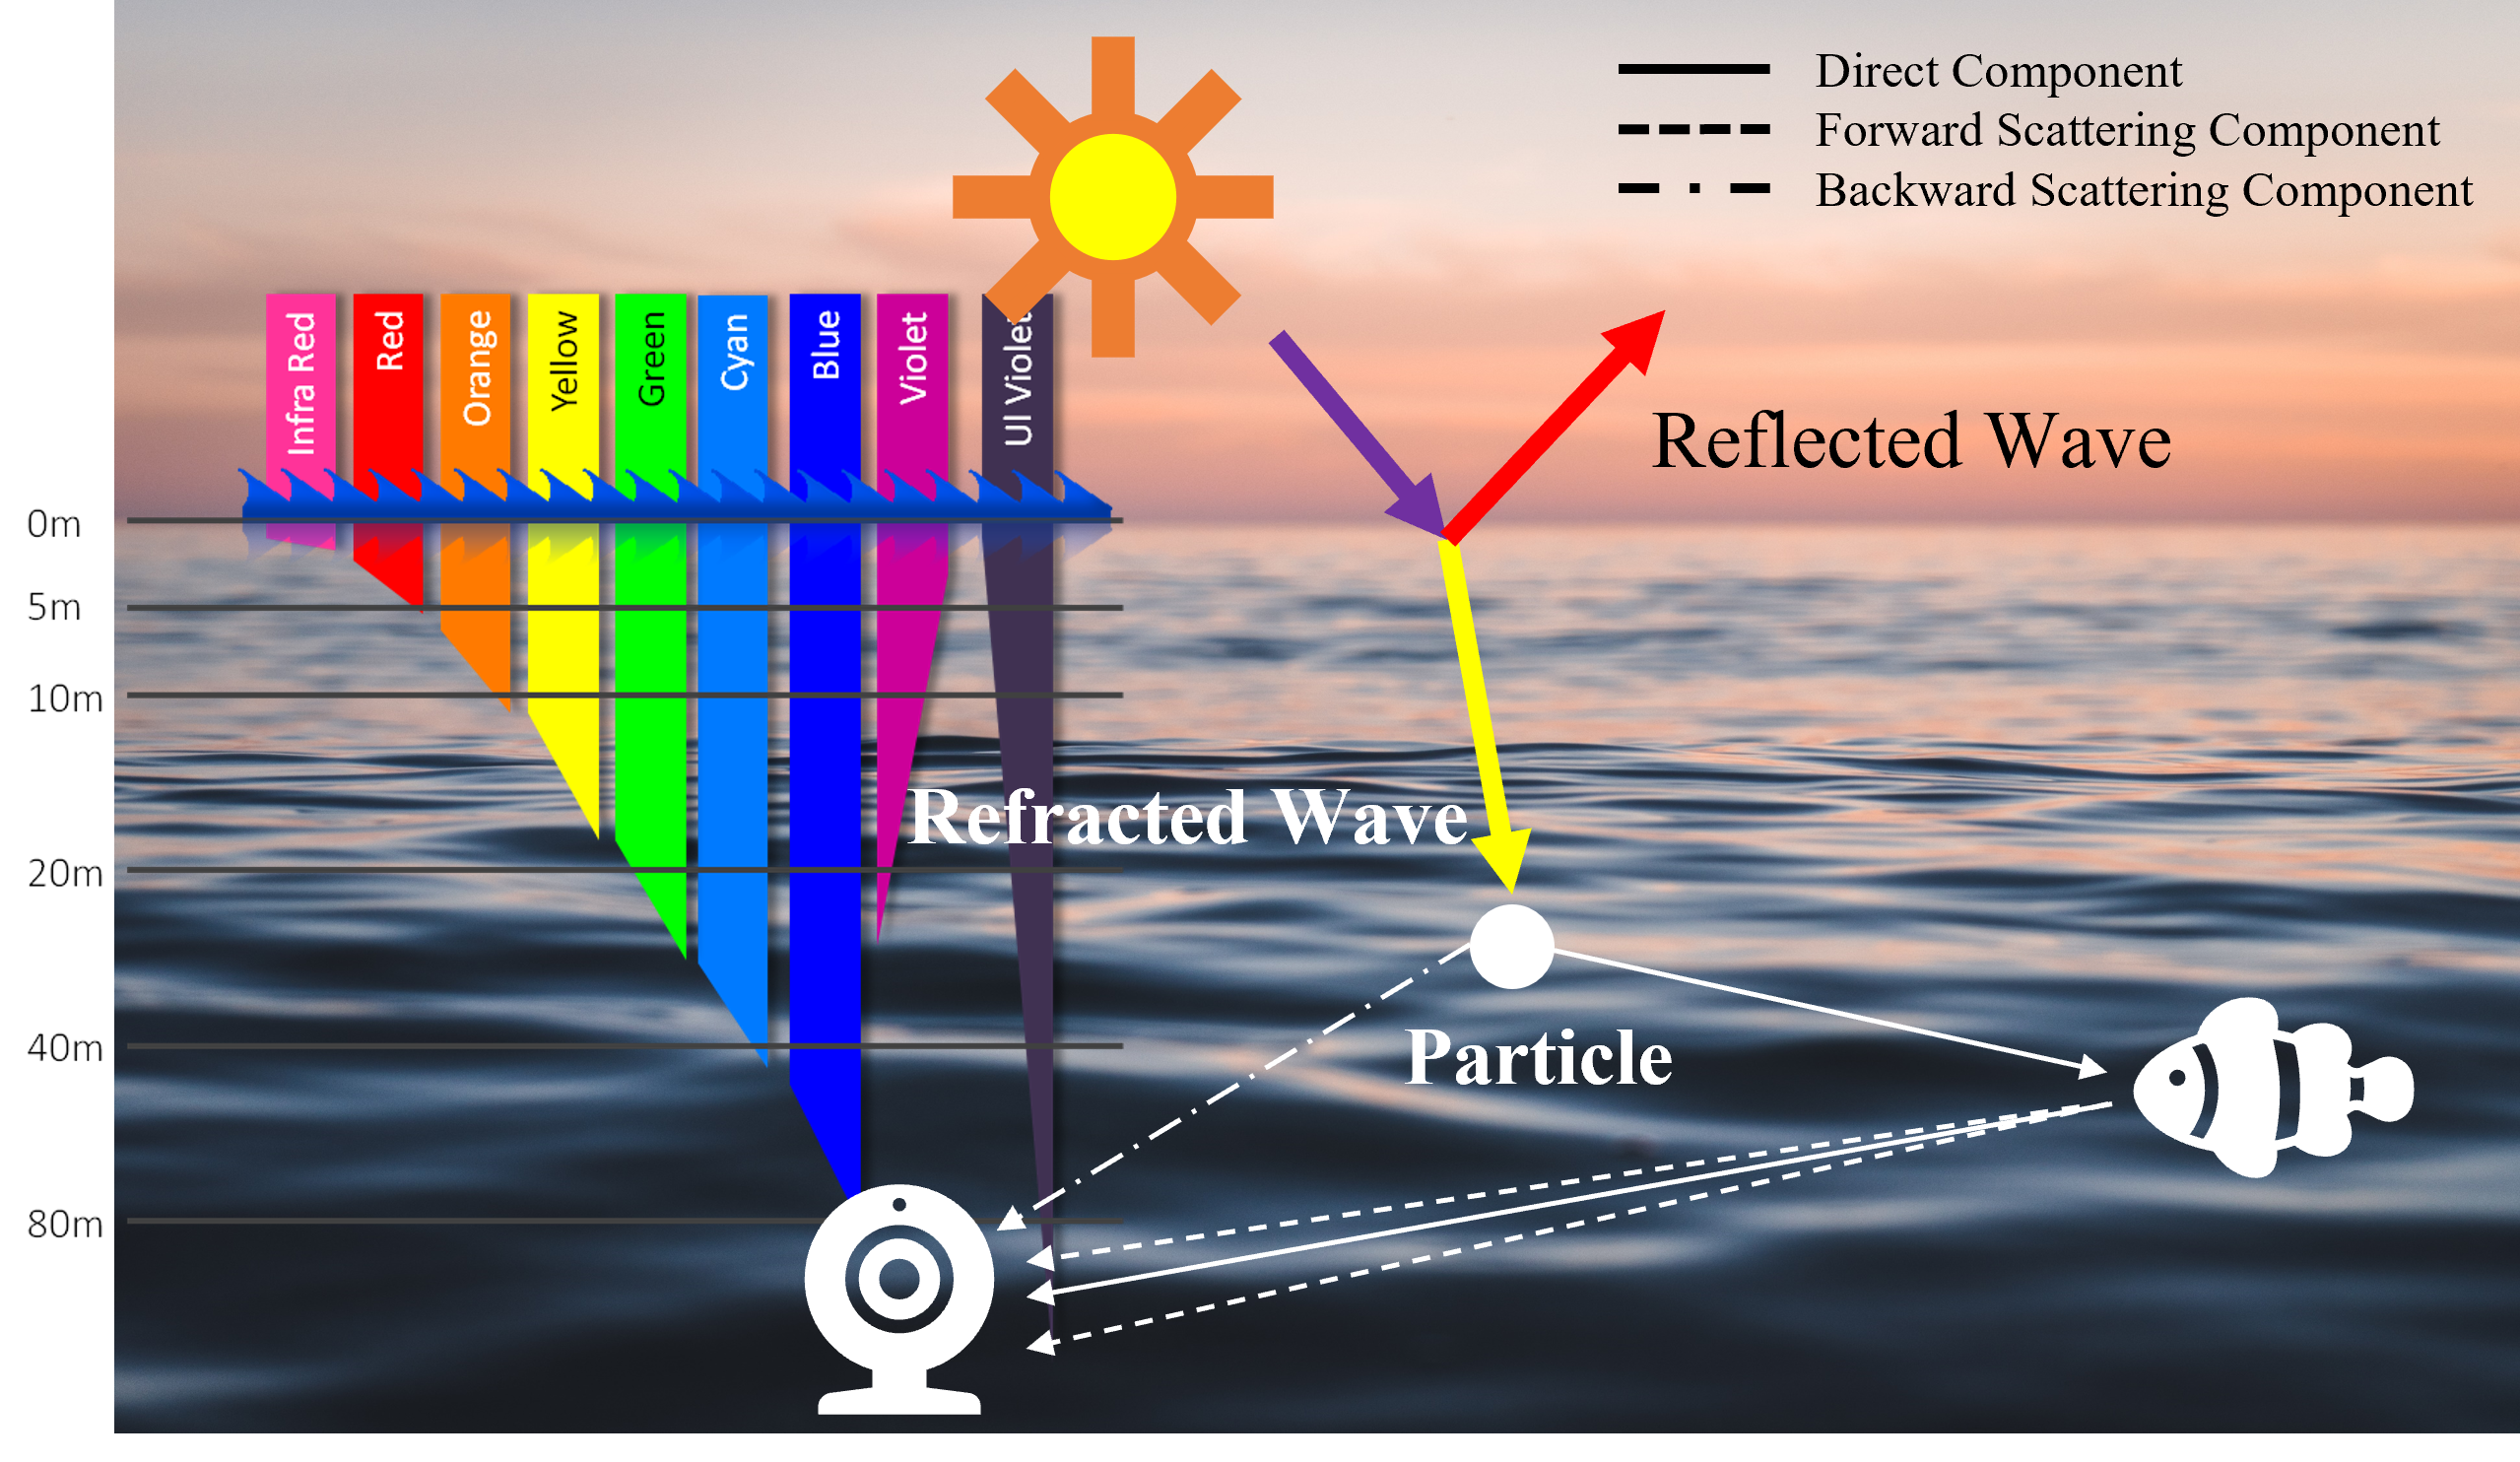
\includegraphics[width=0.45\textwidth]{1_Schematic of Undewater Optical Imaging.png}
\caption{Schematic Of Underwater Image.}
\end{figure}

As stated by Anthony \cite{Seafriends}, some of the reflections are polarised horizontally, while some of them are polarised vertically. With vertical polarisation, objects seem darker and more subdued, making it feasible to capture richer tones that could otherwise be lost in the mix. Seawater is 800 times denser than air, making it a common problem for underwater photography. Thus, light beams from the air are partially reflected and partially absorbed \cite{Seafriends} as they travel to the water.\\
\par
As you get further into the ocean, the amount of light entering the water decreases. Similar to light, water molecules are capable of absorbing part of it. As a result, the underwater sights get darker and darker as the ocean depth increases. The quantity of light beams decreases as you travel deeper, but the colours likewise do so one by one, as their wavelengths decrease \cite{b1}. A depth of 3 meters, for example, causes the colour red to disappear from the sky. Second, the orange hue gradually fades away. At a depth of 5 meters, the orange colour fades away.\\ 
\par
Last but not least, the yellow fades away completely at a depth of 10 meters. \cite{b1} \cite{Seafriends}
To counteract the blue color's dominance, anything submerged changes its natural hue. As a result, blue dominates underwater photographs. Brightness, contrast, and other factors abound in those fuzzy images with lots of blue hues. For underwater photography, our two-step picture improvement approach incorporates white balancing and fusion to improve the images without resorting to an explicit inversion of the optical model. \\
\par
Color casts induced by selective absorption of colours with depth and back scattering are compensated for using white balance and image fusion techniques, respectively in our method of image processing.An in-depth explanation of the fusion process is provided. White-balancing is the next stage we'll focus on.Color casts generated by varying illumination or medium attenuation can be eliminated by the process of white-balancing. Seeing green or blue underwater is a serious issue that must be addressed since it affects depth perception. When light passes through water, the attenuation process affects the wavelength spectrum selectively, affecting both the intensity and appearance of a coloured surface. \\
\par
As we descend into the depths of the ocean, our ability to see colour changes because long-wavelength light is less sensitive to scattering than short-wavelength light. In actuality, the total distance between the observer and the scene has an impact on the attenuation and loss of colour in the image. Many current white balancing techniques have been examined, and a few have been identified that are both successful and suited for our use case.\\ 
\par
After that, we'll quickly go through these strategies and talk about how they inspired the creation of our original undersea approach. Based on a predetermined assumption, these methods estimate the light source colour and then use the normalized light source intensity to ensure colour constancy. As an example, the Gray world method \cite{key:article} assumes that the scene's average reflectance is colourless. Each channel may be averaged to determine how much illuminant light is being dispersed. 

\section{Underwater Image Processing System}

\begin{figure}
\includegraphics[width=0.5\textwidth]{2_Basic Flow Diagram.png}
\caption{Basic Flow Diagram.}
\end{figure}

A two-step procedure, as indicated, is used to improve underwater photographs without explicitly inverting the optical model. The white balancing method we employ seeks to correct the colour cast that results from the selective absorption of colours with depth, while the fusion method we use aims to improve the scene's edges and details while reducing the loss of contrast caused by back scattering. \\

\subsection{White Balancing}
The white-balancing stage is currently our emphasis. By eliminating the unwanted colour casts caused by different lighting or medium attenuation qualities, white-balancing attempts to improve the image's aspect. A major challenge in underwater colour perception is a green-bluish look that needs to be corrected. The attenuation process alters the hue and intensity of a colourful surface by selectively altering the wavelength spectrum when light passes through water (see Section II). 
\\
\par
As we travel deeper into the water, our ability to see colour changes because the scattering weakens long wavelengths more than short ones. Attenuation and loss of colour are also affected by how far away the observer is from the scene they are looking at. We've had a look at a wide range of white balance approaches \cite{key:article}, and we've found some that are both successful and appropriate for our situation (see Fig. 4). Our new solution for underwater scenes is based on the following ideas, which we briefly review and describe below.\\
\par
For underwater scenarios, we observed that the well-known Gray-World method \cite{color constancy} performs well in terms of visual quality. When it comes to significantly damaged underwater scenarios, typical solutions fail miserably, as seen in Figure 4. However, the hue shift remains, and as a result, it seems blue. Although the Grey World approach eliminates the blue tone best, we see strong red artifacts when using it.\\
\par
Overcompensation in areas where red colour is present is caused by a low mean value for the red colour channel (since the Gray world separates each channel by its mean value). It is therefore our primary goal to compensate for the loss of the red channel, as determined by prior underwater studies \cite{Buchsbaum}\cite{drews2013transmission}. Gray World will be used in a second stage to compute the white balance picture.\\

\begin{figure}
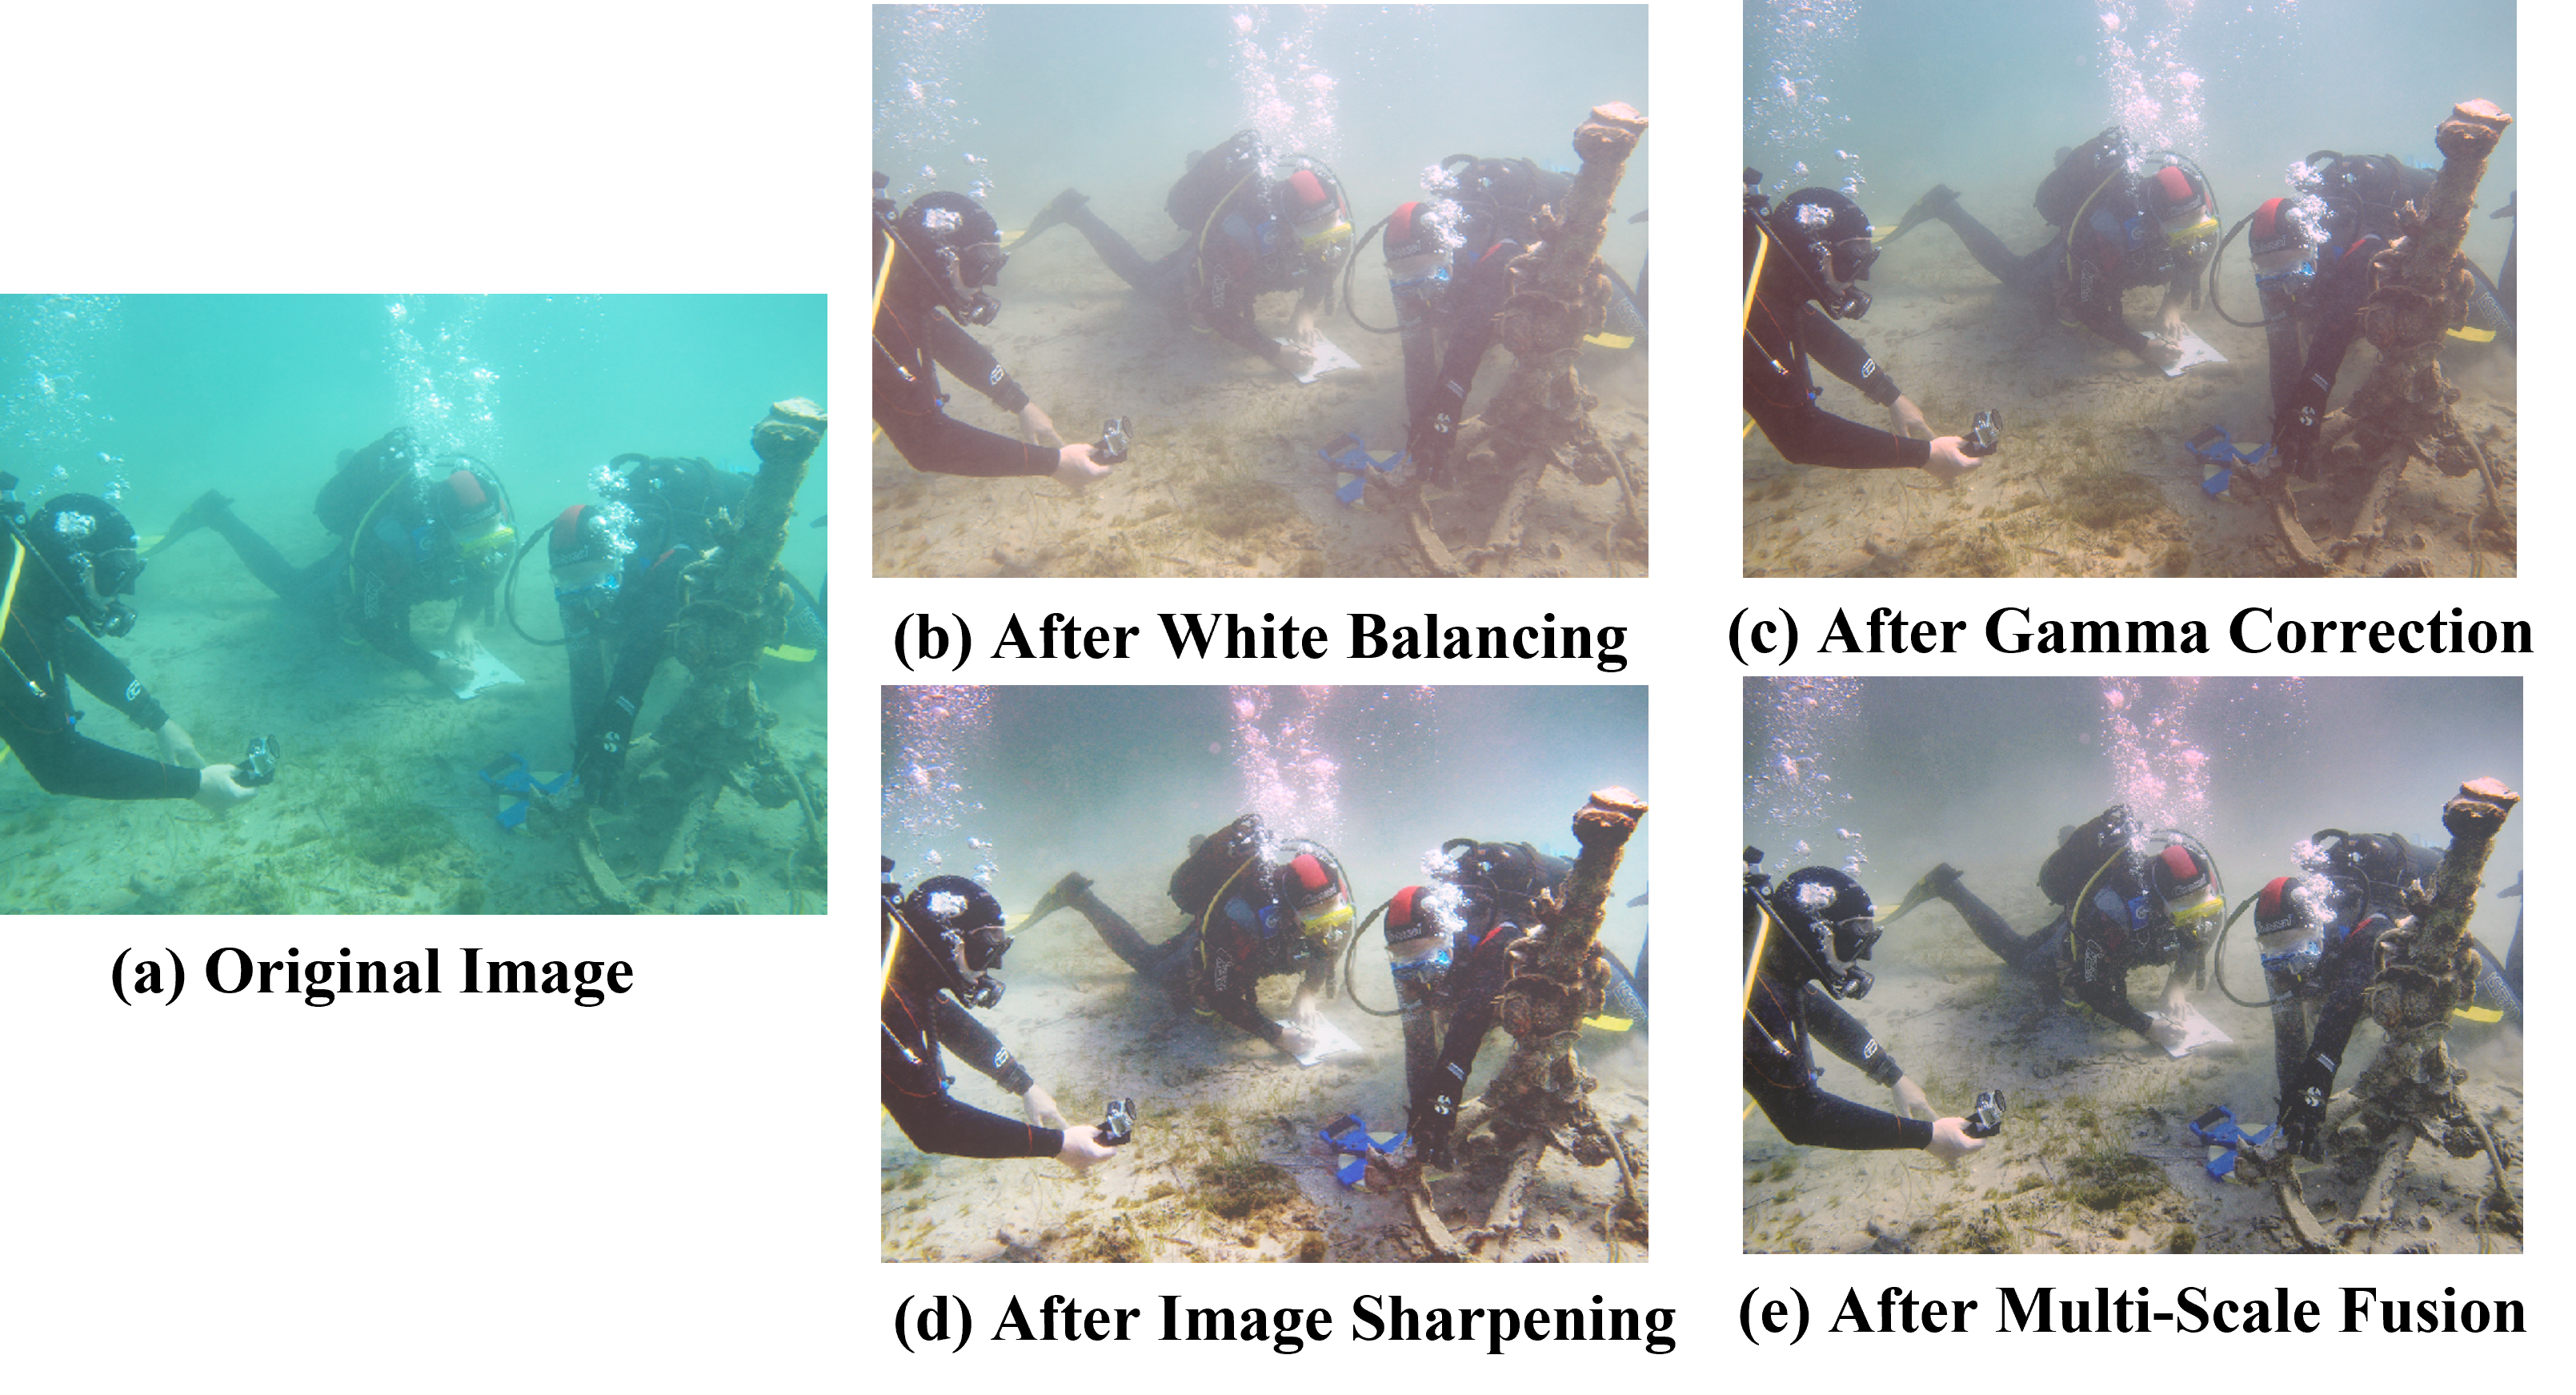
\includegraphics[width=0.5\textwidth]{6_Techniques.png}
\caption{Enhancement Techniques}
\end{figure}

To make up for the absence of the red channel, the following four observations and concepts are employed:\\
1. In comparison to the red and blue channels, the green channel has been retained rather well underwater.\\\par
2. The green channel carries opponent colour information compared to the red channel, and it is thus more crucial to correct for the larger attenuation caused on red, compared to green, when moving in clear water. As a result, a little amount of the green channel is mixed in with the red channel to make up for the red attenuation. \\\par
3. It was initially thought that using both a fraction of green and blue would be the most efficient way to compensate for the loss of colour information in the red channel. Using only the green channel's information allows us to better recover the entire colour spectrum while maintaining a natural appearance of the background (water regions).\\\par
4. Red channel information should not be sent to places where the green channel information is still relevant. Thus, we wish to prevent the reddish colour of the Gray-World method in the over-exposed portions. The red channel must be compensated only in areas where the red channel is severely attenuated (see Fig. 4). A pixel with a significant value for all three channels indicates that it is located near the observer or in an artificially lighted region, and does not need to be restored. This argument follows the statement in \cite{drews2013transmission}.\\\par
We propose to represent the adjusted red channel $I_{rc}$ at each pixel position (x) in this way to account for these observations:\\

\begin{figure}
\includegraphics[width=0.5\textwidth]{8_Before Colour Correction.png}
\caption{Before Colour Correction}
\end{figure}

\begin{figure}
\includegraphics[width=0.5\textwidth]{9_After Colour Correction.png}
\caption{After Colour Correction}
\end{figure}

\begin{figure*}
\includegraphics[width=\textwidth]{7_Overview.png}
\caption{Dehazing strategy summary. Using Gamma correction and edge sharpening, the (too pale) white-balanced picture is split into two separate images, Input 1 and Input 2. Two photos are supplied into the fusion process, which creates weight maps based on normalization and mixes the inputs using a multi-scale method. Multi-scale fusion is demonstrated using only three layers of Laplacian and Gaussian pyramids.}
\end{figure*}

1. For Red Channel Enhancement we perform,

\[I_{rc}(x) = I_r(x) + \alpha.(\Bar{I}_g) - \Bar{I}_r) . (1 - I_r(x)).I_g(x)\]

Color channels of image I's red and green colour channels are represented by $I_g(x)$ and $I_r$  and $I_g$, respectively. A constant parameter is used in above equation to indicate that each element in the second term is a direct outcome of one of the observations listed above. For varied lighting circumstances and acquisition settings, we've found that a = 1 value works well. The unsharp masking notion is what we employ as a consequence.\\

2. For Blue Channel Enhancement,\\
To round out our conversation about the severe and color-dependent dimming of light underwater, it is important to take note of the works in \cite{galdran2015automatic} and \cite{lu2015contrast} \cite{lu2016underwater} \cite{bonin2011imaging}, which uncover and make use of the fact that, in turbid waters or locations with a high concentration of plankton, the blue channel may be significantly dimmed as a result of organic matter's absorption of light. 
\par
These conditions can be found in locations where there is a high concentration of plankton We propose to also compensate for the attenuation of the blue channel to address the situations in which blue is severely attenuated and the compensation of the red channel appears to be insufficient.
\par
To do so, we compute the compensated blue channel $I_{bc}$ using the following formula:

\[I_{bc}(x) = I_b(x) + \alpha.(\Bar{I}_g) - \Bar{I}_b) . (1 - I_b(x)).I_g(x)\]

where $I_b, I_g$ represent the blue and green color channels of image I, and $\alpha$ is also set to one.

\subsection{Multi-Scale Fusion}
We proposed a single picture underwater dehazing technique based on multi-scale fusion concepts in this paper. Picture fusion has been demonstrated to be useful in a variety of applications, including vision compositing \cite{bonin2011imaging}, multispectral video enhancement \cite{grundland2006cross}, defogging \cite{bennett2007multispectral}, \cite{ancuti2013single}, and HDR photography \cite{ancuti2010effective}.\\
\par
We're aiming for a simple and quick solution that can improve scene visibility in such a variety of underwater films and photos. Our system, like those of \cite{bennett2007multispectral} and \cite{ancuti2013single}, is based on a collection of inputs, produced from a single source picture. However, unlike \cite{bennett2007multispectral} and \cite{ancuti2013single}, those two were picked especially to get the most out of the whitebalancing strategy described in the preceding section. A pair of inputs are included to improve the colour contrast and edge sharpness of a white-balanced image, respectively.

\subsection{Inputs of the Fusion Process}
We start by applying our white balance approach to the input images because colour correction is very important underwater. This phase seeks to improve the image's look by removing colour casts created by different illuminants. White balance suffers from obvious impacts at water deeper than 10 feet since the absorbed colours are difficult to restore. As a consequence, we do a gamma correction on the white balanced picture version to produce our initial input.\\
\par
Gamma correction is important since white-balanced underwater photographs tend to seem overly bright in general. This adjustment enhances the contrast between darker and brighter areas at the expense of features in the under- and overexposed areas. We generate a secondary input that relates to a sharper variant of the white balanced image to compensate for this loss.
\par

\begin{table*}[htpb]
\caption{Objective Measurements: Edge and Pixel-based Image quality assessment}
\begin{center}
\resizebox{0.75\textwidth}{!}{
\begin{tabular}{|c|c|c|c|c|c|}
\hline
\textbf{}&\multicolumn{5}{|c|}{Enhancement Techniques} \\
\cline{2-6} 
\textbf{Image Quality} & \textbf{\textit{Original}}& \textbf{\textit{White}}& \textbf{\textit{Gamma}} & \textbf{\textit{Image}}  & \textbf{\textit{Multi-Scale}}\\
\textbf{Matrix} & \textbf{\textit{Image}}& \textbf{\textit{Balancing}}& \textbf{\textit{Correction}} & \textbf{\textit{Sharpening}}  & \textbf{\textit{Fusion}}\\
\hline
%Image Used 6.png
Red Channel &  0.1753 & 0.4962 & 0.2585 & 0.5002 & 0.4226\\
Mean & & & & & \\
\hline
Green Channel &  0.5064 & 0.4886 & 0.2562 & 0.4963 & 0.4191\\
Mean & & & & & \\
\hline
Blue Channel &  0.3092 & 0.4952 & 0.2559 & 0.4996 & 0.4215\\
Mean & & & & & \\
\hline
Peak SNR & $\infty$ & 61.4986 & 64.2340 & 60.4674 & 62.9768\\
 & & & & & \\
\hline
Average &  $\infty$ & 4.8356 & 7.5710 & 3.8044 & 6.3139\\
SNR & & & & & \\
\hline
Structural & & & & & \\
Similarity (SSIM) & 1 & 0.9724 & 0.9947 & 0.9667 & 0.9785\\
Index Value & & & & & \\
\hline
Mean Squared &  0 & 0.2743 & 0.1480 & 0.3319 & 0.2496\\
Error (MSE) & & & & & \\
\hline
No Reference & & & & &\\
Image Quality & 45.1850 & 45.0421 & 44.4191 & 48.4987 & 45.9127 \\
Score & & & & & \\
\hline
\end{tabular}
}
\label{tab1}
\end{center}
\end{table*}

The unsharp masking notion is what we employ as a consequence. The normalized unsharp masking procedure is used to describe the sharpening method. No parameter adjustments are required, and it appears to be effective at sharpening. The addition of this second input significantly reduces the degradation caused by scattering. As a result of the highpass signal emulating the reversal of Laplacian in the second input, the disparity between a white-balanced picture and its Gaussian filtration counterpart causes undesired artifacts \cite{mertens2009exposure}. The multi-scale fusion approach described in the next section will help keep the final blended image free of these artifacts.



\subsection{Hardware Requirements}
The following information pertains to the camera that we utilised:\\
camera format for Image Capturing, The Insta360 brand and model are both types of action cameras. Feature The Resolution4K video recording format has optical image stabilisation as part of its feature set.\\
\par
\textbf{\textit{Specifications:}}\\
4K wide-angle video recording at 60 frames per second, 5.7K panoramic video recording, IPX8 waterproofing, and the ability to capture and utilise 5 metres of bare metal underwater. When a 360-degree panoramic lens and a 4K wide-angle lens are used together, it is possible to record slow motion at a resolution of 3K at 100 frames per second. Even in dim conditions, the night scene mode is still remarkable since it brings out the natural contrast between light and shadow.

\section{RESULTS AND DISCUSSION}
First, we do a thorough validation of the white-balancing method we proposed earlier, then we compare our dehazing method to what's already on the market. Procedures for underwater restoration/enhancement specialized approaches for underwater restoration/enhancement. Finally, we demonstrate the applicability of our method. Segmentation and keypoint matching are two examples of keypoint matching techniques.

\subsection{Subjective Measurements:}
\textbf{1.Red Channel and Blue channel correction}\\
As said earlier we perform the color correction by keeping the value of correction factor-alpha in the range of [0,1]. By this, we can achieve the enhancement of the red channel and the blue channel as shown in Fig 4(b).\\

\textbf{2.Evaluation of white balance & Gamma Correction}\\
In white balance, we concatenate the corrected or enhanced RGB channels and we Linearize gamma-corrected RGB values i.e., the gamma correction of the sRGB values in input so that output contains linear RGB values. Then we estimate the illumination using the Gray-world algorithm afterward we adjust the color balance of the RGB image with chromatic adaption finally once again we Adjust image intensity values or colormap to get the white balanced image which is depicted in Fig 4(c).\\

\textbf{3.Evaluation of Image Sharpening}\\
Here we perform 2-D Gaussian filtering of images by filtering input image with a 2-D Gaussian smoothing kernel with a standard deviation of 0.5 and return the filtered image then we do Normalization and Histogram Equalization This process is done to enhance the contrast of the image. This series of processes is termed Image sharpening and this can be seen in Fig 4(d). \\

\textbf{4.Evaluation of Multi-Scale Fusion}\\
By using the Gaussian Pyramid and the Laplacian Pyramid. An image processing technique known as the Gaussian pyramid breaks an image into smaller and smaller groups of pixels to blur it. The name was inspired by German mathematician Johann Carl Friederich Gauss.\\
\par
Using the Laplacian pyramid, we may assess the degree to which the low-pass filtered image differs from the original MR image. A Laplacian filter is used to calculate a picture's second derivatives, which gauges how quickly the image's first derivatives change. If the values of neighboring pixels are changing, it's because of an edge, but if they're not, it's because of a gradual progression. During the pyramid reconstruction, both Gaussian and Laplacian pyramids contribute to MultiScale fusion. In Fig 7, this may be observed.\\

\section{Conclusion}
We have demonstrated an alternate method for improving the quality of films and still photographs were taken underwater. Our tactic is based on the idea of fusing two or more images into a single new one, and it does not require any other information save the one initial image. \\
\par
In our experiments, we were able to demonstrate that our method can improve a wide variety of underwater images (such as those taken with a variety of cameras, at varying depths, and under a variety of lighting conditions) with a high degree of accuracy, regaining previously lost important features and edges. In addition, we demonstrate for the very first time the usability and significance of the suggested image augmentation approach for a variety of difficult applications involving computer vision in underwater environments.

\bibliography{Bibliography.bib}
\bibliographystyle{plain}
\vspace{12pt}

\end{document}
